\documentclass[russian,utf8,emptystyle]{eskdtext}

\newcommand{\No}{\textnumero} % костыль для фикса ошибки

\ESKDdepartment{Федеральное государственное бюджетное образовательное учреждение высшего профессионального образования}
\ESKDcompany{Московский государственный технический университет им. Н. Э. Баумана}
\ESKDclassCode{23 0102}
\ESKDtitle{Курсовая работа по дисциплине}
\ESKDdocName{<<Эксплуатация АСОИиУ>>}
\ESKDauthor{Гуща~А.~В.}
\ESKDtitleApprovedBy{к.т.н. доцент}{Постников В.М.}
\ESKDtitleAgreedBy{к.т.н. доцент}{Постников В.М.}
\ESKDtitleDesignedBy{Студент группы ИУ5-92}{Гуща~А.~В}

\usepackage{multirow}
\usepackage{tabularx}
\usepackage{tabularx,ragged2e}
\usepackage{pdfpages}
\renewcommand\tabularxcolumn[1]{>{\Centering}p{#1}}
\newcommand\abs[1]{\left|#1\right|}

\usepackage{longtable,tabu}

\usepackage{geometry}
\geometry{footskip = 1cm}

\pagenumbering{arabic}
\pagestyle{plain}

\usepackage{setspace}
\usepackage{enumitem}

\usepackage{xcolor}
\usepackage{listings}
\lstset{
    breaklines=true,
    postbreak=\raisebox{0ex}[0ex][0ex]{\ensuremath{\color{red}\hookrightarrow\space}},
    extendedchars=\true,
    basicstyle=\small,
    inputencoding=utf8
}
\lstdefinelanguage{D}{
    keywords = {
    abstract,
    alias,
    align,
    asm,
    assert,
    auto,
    body,
    bool,
    break,
    byte,
    case,
    cast,
    catch,
    cdouble,
    cent,
    cfloat,
    char,
    class,
    const,
    continue,
    creal,
    dchar,
    debug,
    default,
    delegate,
    delete,
    deprecated,
    do,
    double,
    else,
    enum,
    export,
    extern,
    false,
    final,
    finally,
    float,
    for,
    foreach,
    foreach_reverse,
    function,
    goto,
    idouble,
    if,
    ifloat,
    immutable,
    import,
    in,
    inout,
    int,
    interface,
    invariant,
    ireal,
    is,
    lazy,
    long,
    macro,
    mixin,
    module,
    new,
    nothrow,
    null,
    out,
    override,
    package,
    pragma,
    private,
    protected,
    public,
    pure,
    real,
    ref,
    return,
    scope,
    shared,
    short,
    static,
    struct,
    super,
    switch,
    synchronized,
    template,
    this,
    throw,
    true, 
    try,
    typedef,
    typeid,
    typeof,
    ubyte,
    ucent,
    uint,
    ulong,
    union,
    unittest,
    ushort,
    version,
    void,
    volatile,
    wchar,
    while,
    with,
    __FILE__,
    __MODULE__,
    __LINE__,
    __FUNCTION__,
    __PRETTY_FUNCTION__,
    __gshared,
    __traits,
    __vector,
    __parameters,
    }
}

\begin{document}
\maketitle
%\includepdf[pages={1}]{title.pdf}

\section{Реферат}
Данный документ представляет собой расчетно-пояснительную записку к курсовой работе по курсу «Эксплуатация АСОИиУ».

Целью курсовой работы является разработка проектного решения на распределенную систему обработки данных (РСОД), объединяющую центральный офис и два удаленных филиала фирмы. В процессе выполнения курсовой работы предстоит решить следующие задачи:
\begin{itemize}[label=-]
\item Выбор сетевого, телекоммуникационного оборудования и программного обеспечения для РСОД.
\item Настройка рабочих параметров сетевой ОС и СУБД.
\item Распределение предметных баз данных (ПБД) по узлам сети.
\item Предложены возможные варианты для модернизации и реорганизации корпоративной сети фирмы.
\item Аналитическое и имитационное моделирование РСОД.
\end{itemize}

Графическая часть содержит следующие материалы:
\begin{itemize}[label=-]
\item Структурные схемы ЛВС центрального и удаленных филиалов фирмыи организации их удаленной связи (лист 1).
\item Исходные данные и окончательные  варианты распределения предметных баз данных по узлам сети (лист 2).
\item Структурная схема моделируемой сети, исходные данные и результаты моделирования (лист 3).
Листы выполнены в виде плакатов.
\end{itemize}

\clearpage

\tableofcontents
\clearpage

\section{Техническое задание}
Исходные данные для выполнения курсовой работы представлены в таблице~\ref{tab:task}.

\begin{longtable}{p{1cm}|p{2cm}|p{2cm}|p{2cm}|p{2cm}|p{2cm}|p{1.5cm}|p{1.5cm}}
\caption{Исходные данные для выполнения курсовой работы.}
\label{tab:task} \\
№  & Цент-ральный офис & 1-ый филиал & 2-ой филиал & СУБД и выбор оборудования & Диски сервера & Диски сервера & Модель \\ 
\hline 
8 & 5(1)/2(1) & 3(3)/2(3) & \centering 18 & 23/33/43 & \centering 53 & 64 (5) (0.9) & \centering 73 \\ 
\end{longtable}

\subsection{Наименование}
Проектирование распределённой АСОИиУ фирмы.

\subsection{Основание для разработки}
Основанием для разработки является учебный план кафедры ИУ5 МГТУ им. Н.Э. Баумана.

\subsection{Цель разработки}
Целью разработки является создание проектного решения на распределенную сеть обра-
ботки информации, объединяющую все подразделения фирмы, состоящей из центрального и двух
удаленных офисов.

\subsection{Задачи, подлежащие решению}
В процессе выполнения курсовой работы необходимо решить следующие задачи:
\begin{enumerate}[label=\arabic*.]
\item Разработать блок-схему распределенной АСОИиУ фирмы и структурные схемы ЛВС цен-
трального и удаленных офисов фирмы;
\item Описать правила построения всех сетей фирмы;
\item Выбрать и обосновать вариант удаленной связи отдельных ЛВС фирмы;
\item Выбрать требуемое оборудование для ЛВС фирмы;
\item Описать настройку рабочих параметров сетевой ОС, под управлением которой работают ЛВС
фирмы;
\item Описать настройку рабочих параметров СУБД, которая установлена в ЛВС фирмы;
\item Провести распределение предметных баз данных по узлам сети;
\item Выполнить аналитическое и имитационное моделирование ЛВС фирмы и провести сравни-
тельный анализ результатов моделирования;
\item Разработать и представить рекомендации по модернизации и реорганизации распределенной
АСОИиУ фирмы.
\end{enumerate}


\subsection{Требования к составу технических средств}
Фирма состоит из центрального офиса и двух филиалов.

В центральном офисе фирмы расположены ЛВС 100Base-TX, содержащая один концетратор, и ЛВС 10Base-2, содержащая один сегмент. Обе сети подключены к коммутатору, к нему также подключен удаленный маршрутизатор с двумя модемами. 

В первом филиале фирмы расположены ЛВС 10Base-T, содержащая 3 концетратора, и ЛВС 10Base-2, содержащая 3 сегмента. Обе сети подключены к коммутатору, к нему также подключен удаленный маршрутизатор с одним модемом.

Во втором филиале фирмы расположена ЛВС Token Ring на комбинированной среде (ВОЛС (волоконно-оптическая линия связи) и ЭВП (экранированная витая пара)). 

\subsection{Требования к составу программных средств}
ЛВС работает под управлением сетевой ОС Windows Server 2003 и СУБД SQL Server. 

\subsection{Техническая документация, предъявляемая по окончанию работы}
По окончании работы должна быть предъявлена следующая документация:
\begin{enumerate}[label=-]
\item структурная схема объединённой сети фирмы;
\item распределение предметных баз данных по узлам сети;
\item формализованная схема сети и результаты моделирования;
\item пояснительная записка.
\end{enumerate}

\subsection{Порядок приема работы}
Приём работы осуществляется путем проверки соответствия выполненной работы пунктам
технического задания.

\subsection{Дополнительные условия}
В ЛВС установлен сервер на базе двухядерного процессора с дисковой подсистемой RAID-6, содержащая 5 базовых диска (без учета уровня RAID), при условии, что вероятность безотказной работы одного диска равна 0.9 и все диски одинаковые.

Необходимо провести сравнительный анализ серверов отдела на базе двухядерных процессоров  и выбрать наилучший.

Подробно описать особенности эксплуатации  системного блока сервера.

Провести моделирование системы, содержащей ПЭВМ,канал и два сервера. Модель должна позволять проводить ее настройку на два варианта:
\begin{itemize}
\item на общий вид моделируемой ЛВС, чтобы можно было провести исследование любого варианта;
\item на вариант задания (исходные данные - только данные задания). 
\end{itemize}

Результаты моделирования должны соответствовать варианту задания, поэтому  необходимо провести  моделирование системы, содержащей 8 рабочих станций, ПЭВМ, канал и два сервера.

\clearpage
\section{Архитектура объединенной сети фирмы}
\subsection{Общая схема сети}
Объединенная сеть состоит из сети центрального офиса, сети 1 филиала и сети 2 филиала. Её общая схема изображена на рисунке~\ref{fig:network-all}. В графических обозначениях схема изображена на рисунке~\ref{fig:network-all-2}.

\begin{figure}[h!]
\centering
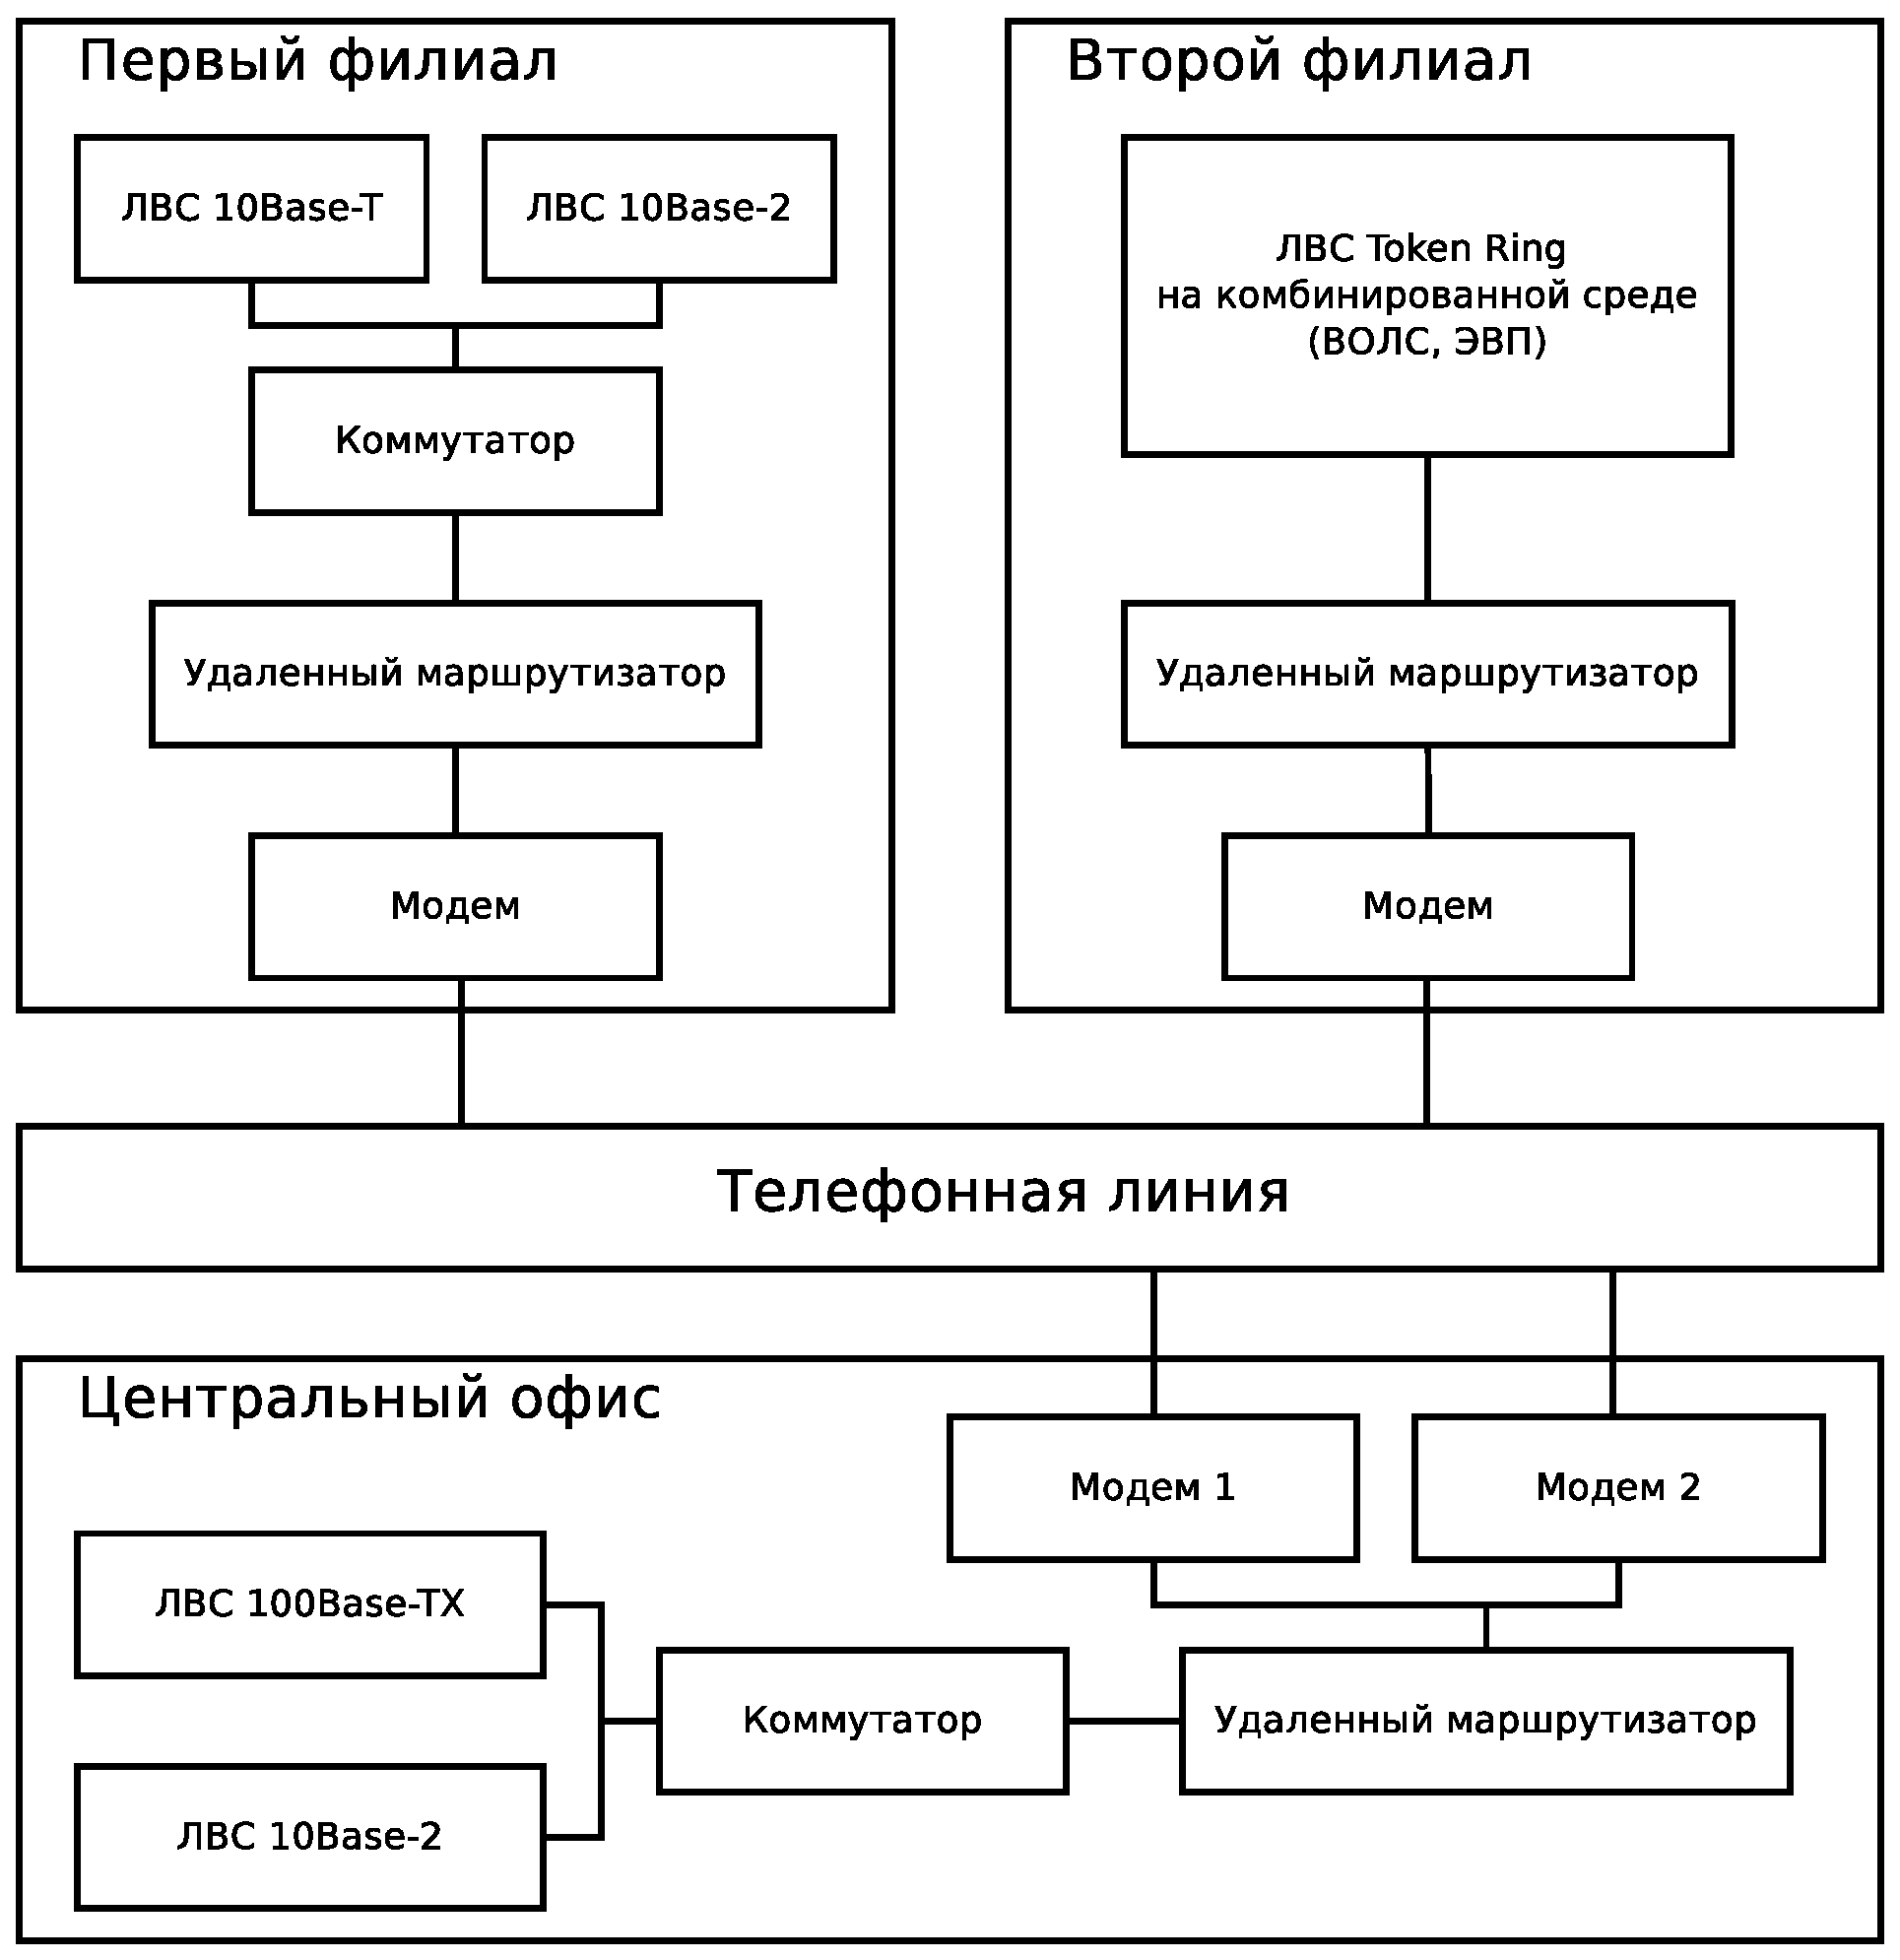
\includegraphics[width = 0.8\textwidth]{network-all}
\caption{Общая схема объединенной сети.}
\label{fig:network-all}
\end{figure}

В центральном офисе фирмы расположены ЛВС 100Base-TX и ЛВС 10Base-2. Обе сети подключены к коммутатору, к которому также подключён удаленный маршрутизатор с двумя модемами.

В первом филиале фирмы расположены ЛВС 10Base-T и ЛВС 10Base-2. Обе сети подключены к коммутатору, к нему также подключен удаленный маршрутизатор с одним модемом.

Во втором филиале фирмы расположена ЛВС Token Ring на комбинированной среде (ВОЛС и ЭВП).

\begin{figure}[h!]
\centering
\includegraphics[width = 0.8\textwidth]{network-all-2}
\caption{Общая схема объединенной сети в графических обозначениях.}
\label{fig:network-all-2}
\end{figure}

\clearpage
\subsection{Схема сети центрального офиса}
В центральном офисе расположены ЛВС 100Base-TX, содержащая один концентратор, и ЛВС 10Base-2, содержащая один сегмент. Обе сети подключены к коммутатору, к нему также подключены удаленный маршрутизатор с двумя модемами. В главном офисе расположен сервер фирмы. Схема сети представлена на рисунке~\ref{fig:main-ofice}.

\begin{figure}[h!]
\centering
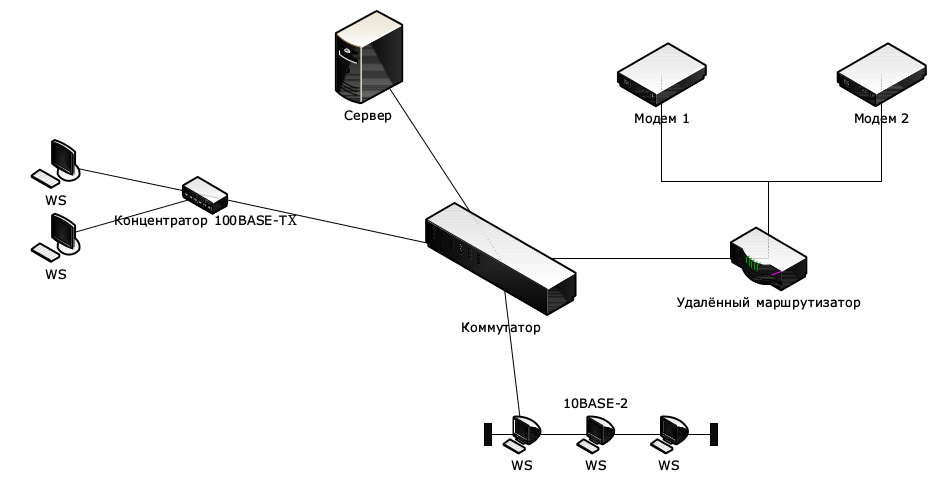
\includegraphics[width=0.8\textwidth]{main_ofice}
\caption{Схема сети центрального офиса.}
\label{fig:main-ofice}
\end{figure}
Во втором филиале фирмы расположена ЛВС Token Ring на комбинированной среде (ВОЛС (волоконно-оптическая линия связи) и ЭВП (экранированная витая пара)). 
\clearpage
\subsection{Схема сети первого филиала}
В первом филиале фирмы расположены ЛВС 10Base-T, содержащая 3 концетратора, и ЛВС 10Base-2, содержащая 3 сегмента. Обе сети подключены к коммутатору, к нему также подключен удаленный маршрутизатор с одним модемом. Схема сети прдеставлена на рисунке~\ref{fig:filial-ofice-1}.

\begin{figure}[h!]
\centering
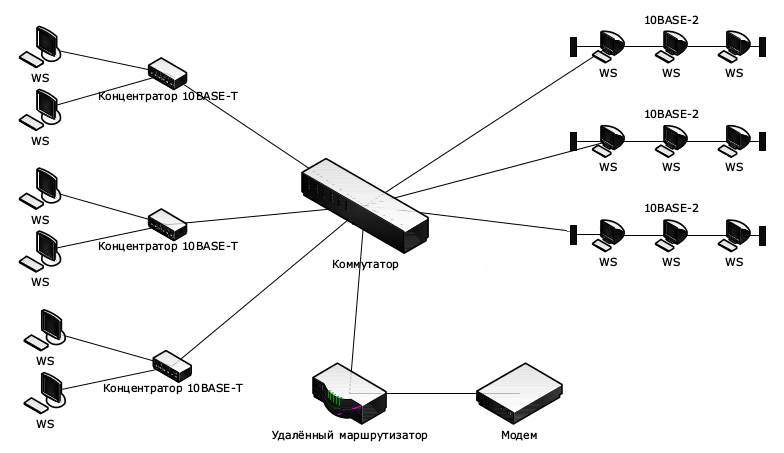
\includegraphics[width=0.8\textwidth]{filial_ofice_1}
\caption{Схема сети первого филиала.}
\label{fig:filial-ofice-1}
\end{figure}


\clearpage
\subsection{Схема сети второго филиала}
Во втором филиале фирмы расположена ЛВС Token Ring на комбинированной среде (ВОЛС (волоконно-оптическая линия связи) и ЭВП (экранированная витая пара)). Схема сети прдеставлена на рисунке~\ref{fig:filial-ofice-2}.

\begin{figure}[h!]
\centering
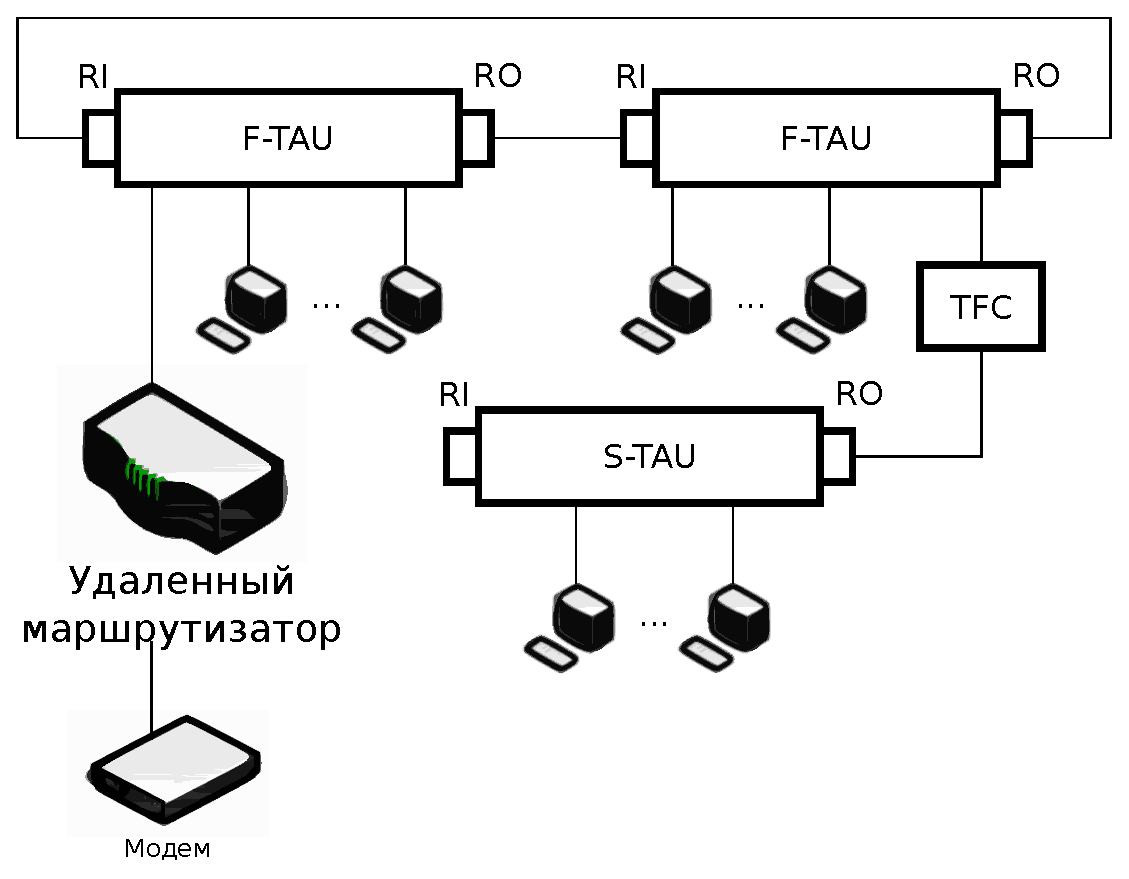
\includegraphics[width=0.8\textwidth]{filial_ofice_2}
\caption{Схема сети второго филиала.}
\label{fig:filial-ofice-2}
\end{figure}

\clearpage
\subsection{Правила построения сети}
Для построения работоспособной сети следует придерживаться ряда правил.

\subsubsection{Правила построения сетей 100Base-TX}
Для построения сети на основе 100Base-TX применяются следующие правила:
\begin{itemize}[label=-]
\item используется витая пара 5 категории;
\item в кабеле используются только 2 пары;
\item длина луча сети должна быть не более 100 метров;
\item между двумя узлами сети расстояние не может быть больше 205 м;
\item между любыми двумя узлами должно быть не более 5 сегментов и 4 повторителей;
\end{itemize}

\subsubsection{Правила построения сетей 10Base-T}
При построении сети на основе 10BaseT применяются следующие правила:
\begin{itemize}[label=-]
\item длина сегмента – 100 метров;
\item между двумя узлами может быть не выше 5 лучей;
\item общее количество станций не должно превышать 1024;
\item максимальное число концентраторов между любыми двумя станциями сети - 4;
\item максимальный диаметр сети - 500 м;
\item используются коннекторы RJ-45;
\item не допускается образование колец;
\item используется неэкранированная витая пара 3 категории.
\end{itemize}

\subsubsection{Правила построения сетей 10Base-2}
При построении сети на основе 10Base2 применяются следующие правила:
\begin{itemize}[label=-]
\item используется тонкий коаксиальный кабель с терминаторами на обоих концах;
\item для усиления сигнала используются повторители;
\item повторители должны быть подключены к источнику электропитания;
\item рабочие станции подключаются к кабелю с помощью сетевых адаптеров с разъёмом BNC и T-коннекторов;
\item один из терминаторов каждого сегмента заземляется;
\item T-коннектор подключается к терминатору непосредственно или через расстояние кратное 2.5 м;
\item минимальное расстояние между двумя Т-коннекторами составляет 2.5 м;
\item расстояние между двумя Т-коннекторами должно быть кратно 2.5 м;
\item между любыми двумя узлами должно находиться не более 5 сегментов, 4 повторителей;
\item длина сегмента не более 185 м;
\item длина сети не более 925 м;
\item к сегменту может быть подключено не более 30 узлов.
\end{itemize}

\subsubsection{Правила построения сетей Token Ring}
При построении сети на основе Token Ring ЭВП и ВОЛС применяются следующие правила:
\begin{itemize}[label=-]
\item в качестве кабеля используется экранированная витая пара (ЭВП) для S-TAU и волоконно оптические линии связи (ВОЛС) для F-TAU;
\item для доступа к сети используется F-TAU и S-TAU;
\item максимум в сети может быть не больше 255 узлов;
\item для точки соединения между средами передачи сигнала используется TFC (Token ring optic Fiber Converter);
\item максимальное расстояние между устройствами доступа S-TAU составляет 100 м, между устройствами доступа F-TAU 3000 м;
\end{itemize}

\clearpage
\section{Построение сети}
\subsection{Принципы построения производительных сетей}

Производительность системы определяется сочетанием её аппаратно- программных средств.
Повышение производительности может быть достигнуто путем использования аппаратных средств,
обладающих лучшими характеристиками производительности по сравнению с уже применяющи-
мися.

Повышение производительности сервера, следует производить в соответствии с предвари-
тельными расчетами <<узких мест>> – аналитическими расчетами, либо с помощью моделирования
его работы. Эти расчеты показывают целесообразность увеличения производительности того или
иного узла сервера - процессора, дисковой подсистемы. Аналогично для ЛВС можно определить,
например, актуальность увеличения пропускной способности каналов связи.

Производительность сервера зависит от наличия:
\begin{itemize}[label=-]
\item количества центральных процессоров;
\item шин PCI и их большой производительности;
\item большого объема памяти ОЗУ;
\item высокоскоростного дискового интерфейса;
\item организация дисковых подсистем с использованием RAID, обеспечивающих увеличение производительности.
\end{itemize}


\subsection{Принципы построения отказоустойчивых сетей}
Отказоустойчивость сети определяется двумя факторами:
\begin{itemize}[label=-]
\item уровень избыточности сетевой инфраструктуры;
\item время восстановления сети, то есть время, необходимое для переключения потоков данных
на работоспособные части сети в случае отказа ее части.
\end{itemize}

При построении отказоустойчивой системы необходимо учесть следующее:
\begin{enumerate}[label=\arabic*.]
\item Архитектура сетевого оборудования:
\begin{itemize}[label=-]
\item дублирование блоков питания;
\item возможность "горячей"замены компонентов;
\item дублирование управляющего модуля;
\item дублирование коммутационной матрицы/шины.
\end{itemize}

\item Дублирование соединений:
\begin{itemize}[label=-]
\item использование нескольких дублирующих соединений;
\item не рекомендуется использовать протокол Spanning Tree, так как в сети появляется много
неработающих (заблокированных) соединений, а время восстановления очень большое;
\item желательно использовать технологии Multi-Link Trunk (MLT) и Split-MLT (автоматиче-
ская балансировка потоков данных между всеми работоспособными соединениями; вос-
становление сети за доли секунды);
\item возможно внедрение протоколов балансировки нагрузки и дублирования на уровне марш-
рутизации;
\item разнесение окончания каналов - окончание каналов на разных модулях ввода/вывода
и/или на разных узлах для дополнительного дублирования;
\item разнесение каналов - использование различных носителей и различных путей для кри-
тичных соединений;
\end{itemize}

\item Высоконадежное сетевое оборудование - устройства с высоким временем наработки на отказ;
\item Отказоустойчивость сервера:
\begin{itemize}[label=-]
\item использование технологии PCI Hot Plug замены отдельных узлов;
\item многопроцессорные серверы;
\item организация дисковых подсистем с использованием RAID, обеспечивающих увеличение
надежности;
\item дублирование дискового контроллера RAID;
\item дублирование сетевых адаптеров;
\item установка резервных вентиляторов для охлаждения процессора, ОЗУ, дисков, плат;
\item организация резервного электропитания центрального процессора;
\item резервирование источников питания;
\item съемная плата кэш-памяти для диска со встроенной батареей;
\item наличие заводского ВIOS (ПЗУ) и рабочего BIOS (ППЗУ).
\end{itemize}

\end{enumerate}

\clearpage
\subsection{Расчет вероятности безотказной работы дисковой подсистемы сервера}
Согласно ТЗ, необходимо определить вероятность безотказной работы дисковой подсисте-
мы сервера, построенной на базе RAID-6, содержащей 5 базовых диска (без учета уровня RAID),
при условии, что вероятность безотказной работы одного диска равна 0.9 и все диски одинаковые.

RAID 6 имеет высокую степень надёжности — под контрольные суммы выделяется ёмкость
2 дисков, рассчитываются 2 суммы по разным алгоритмам. Обеспечивает работоспособность после
одновременного выхода из строя двух дисков — защита от кратного отказа. То есть, массив выходит
из строя только при отказе трёх и более дисков. Схема дискового массива RAID-6 представлена на рисунке~\ref{fig:raid-6}.

\begin{figure}[h!]
\centering
\includegraphics[width=0.8\textwidth]{raid-6}
\caption{Схема дискового массива RAID-6.}
\label{fig:raid-6}
\end{figure}

Вероятность безотказной работы массива RAID-6 для $n$ дисков определяется по следующей формуле:
$$
P = p^n + n(1-p)p^{n-1} + {n \choose 2}(1-p)^2 p^{n-2}
$$
Количество сочетаний вычисляется по следующей формуле:
$$
{n \choose k} = \frac{n!}{k!(n-k)!}
$$

Для $n=5$ и $p=0.9$ получаем следующую формулу:
\begin{align} \label{eq:raid-6}
P & = 0.9^5 + 5*0.1*0.9^4 + {5 \choose 2}*0.1^2*0.9^3 \\
  & = 0.59049 + 0.32805 + 10*0.00729 = 0.99144
\end{align}

Вероятность безотказной работы дисковой подсистемы сервера на базе RAID-6 согласно формуле~\ref{eq:raid-6} равняется 0.99144.

\subsection{Рекомендации по модернизации сети}
В центральном офисе и в первом филиале в сети используются устаревшие технологии: 10BASE-T и 10BASE-2. И если первую ещё можно модернизировать путём замены сетевых адаптеров и концентраторов с возможностью использования уже проложенного кабеля, то вторая потребует ещё и замены всего оборудования плюс демонтаж старого и прокладку нового кабеля.

Если для работы фирмы достаточно текущей скорости передачи данных в сети и её пропускной способности, то не рекомендуется проводить модернизацию, так как это выльется в существенные финансовые и временные затраты.

\clearpage
\section{Организация связи с филиалами}
\subsection{Выбор технологии}
Мною было рассмотрено три варианта организации удалённых связей сети фирмы: VPN через Интернет, Frame Relay и ADSL.

VPN (Virtual Private Network — виртуальная частная сеть) - является современным способом создавать дешевые и защищенные каналы передачи данных между локальными сетями через сеть Интернет. Вместо модемов используются аппаратные или программные шлюзы, подключенные к сети Интернет. Данный подход позволяет сократить затраты на подключение, так как филиалы и главный офис разделяют соединение к сети Интернет вместе с виртуальными каналами VPN.

Стоимость организации VPN сети в среднем составляет 10 000 р., в которую входят стоимость аппаратного обеспечения и настройки программного обеспечения. Абонентская плата для скорости 10 Мбит/с составляет 2 700 р. в месяц.

Сети Frame Relay - сравнительно новые сети, которые гораздо лучше подходят для передачи пульсирующего трафика локальных сетей по сравнению с сетями Х.25. Преимущество сетей Frame Relay заключается в их низкой протокольной избыточности и дейтаграммном режиме работы, что обеспечивает высокую пропускную способность и небольшие задержки кадров. Надежную передачу кадров технология Frame Relay не обеспечивает. Сети Frame Relay специально разрабатывались как общественные сети для соединения частных локальных сетей. Они обеспечивают скорость передачи данных до 2 Мбит/с.

Сети Frame Relay следует применять только при наличии на магистральных каналах волоконнооптических кабелей высокого качества. Стоимость использования данной сети достаточно высока. Подключение стоит 57000 рублей и абонентская плата составляет 9000 рублей в месяц.

ADSL модемы передают данные намного быстрее, чем обычные аналоговые модемы, используя те же телефонные линии. ADSL обеспечивает высокоскоростной широковещательный доступ. Скорость передачи данных достигает 6 Мб/с. ADSL работает по имеющейся телефонной
линии и при этом не занимает телефонный канал. Таким образом, возможно одновременно пользоваться телефонным аппаратом и осуществлять доступ в интернет. Фактически, ADSL модем образует три канала:
\begin{itemize}[label=-]
\item входящий канал, скорость до 6 Мбит/с,
\item исходящий канал, скорость до 1 Мб/с,
\item обычный канал телефонной связи, по которому ведутся телефонные разговоры.
\end{itemize}

Скорость передачи данных зависит от используемого оборудования, длины и качества телефонной линии. ADSL не требует, как аналоговый модем, набора номера для установления соединения с сетью. Обычно, телефонные сервисы используют минимальную часть пропускной способности телефонной линии, ADSL занимает оставшуюся часть для реализации высокоскоростной передачи данных. Подключение стоит 3 000 рублей, а абонентская плата составляет 2 500 рублей в месяц.

Качественные характеристики рассматриваемых технологий сведены в таблицу~\ref{tab:connect-1}.

\begin{longtable}{p{7cm}|p{2cm}|p{2cm}|p{2cm}}
\caption{Качественные характеристики технологий передачи данных}
\label{tab:connect-1} \\
Параметр  & VPN & Frame Relay & ADSL \\ 
\hline 
Скорость передачи, Мб/c     & 10 & 2 & 6  \\ 
Надёжность передачи данных & Отличная & Отличная & Хорошая  \\ 
Возможность масштабирования & Хорошая & Отличная & Плохая  \\ 
Стоимость подключения, рублей & 10 000 & 57 000 & 3 000  \\ 
Абонентская плата, рублей & 2 700 & 9 000 & 2 500 \\
\end{longtable}

Количественные характеристики рассматриваемых технологий сведены в таблицу~\ref{tab:connect-2}.

\begin{longtable}{p{7cm}|p{2cm}|p{2cm}|p{2cm}}
\caption{Количественные характеристики технологий передачи данных}
\label{tab:connect-2} \\
Параметр  & VPN & Frame Relay & ADSL \\ 
\hline 
Скорость передачи, Мб/c     & 10 & 2 & 6  \\ 
Надёжность передачи данных & 5 & 5 & 4  \\ 
Возможность масштабирования & 4 & 5 & 2  \\ 
Стоимость подключения, рублей & 10 000 & 57 000 & 3 000  \\ 
Абонентская плата, рублей & 2 700 & 9 000 & 2 500 \\
\end{longtable}

Теперь пронормируем параметры и добавим весовые коэффициенты. Результаты приведены в таблице~\ref{tab:connect-3}.

\begin{longtable}{p{7cm}|p{1cm}|p{2cm}|p{2cm}|p{2cm}}
\caption{Расчет весовых коэффицентов технологий передачи данных}
\label{tab:connect-3} \\
Параметр & $\alpha$ & VPN & Frame Relay & ADSL \\ 
\hline 
Скорость передачи, Мб/c      & 0.3 & 1    & 0.2  & 0.6   \\ 
Надёжность передачи данных   & 0.3 & 1    & 1    & 0.8   \\ 
Возможность масштабирования  & 0.2 & 0.8  & 1    & 0.4   \\ 
Стоимость подключения, рублей& 0.1 & 0.3  & 0.05 & 1     \\ 
Абонентская плата, рублей    & 0.1 & 0.93 & 0.28 & 1     \\
\hline
Итог                         & 1.0 & 0.88 & 0.59 & 0.7
\end{longtable}

Согласно таблице~\ref{tab:connect-3} необходимо выбрать VPN. 

\clearpage
\subsection{Выбор оборудования}
\subsubsection{Выбор маршрутизатора}

Выбираем из трех маршрутизаторов:
\begin{enumerate}[label=\arabic*.]
\item ASUS RT-N10P
\item TP-LINK TL-R470T+
\item D-link DIR-100
\end{enumerate}

Качественные характеристики рассматриваемых маршрутизаторов сведены в таблицу~\ref{tab:routers-1}.

\begin{longtable}{p{7cm}|p{2cm}|p{2cm}|p{2cm}}
\caption{Качественные характеристики рассматриваемых маршрутизаторов}
\label{tab:routers-1} \\
Параметр                     & ASUS RT-N10P & TP-LINK TL-R470T+ & D-link DIR-100 \\ 
\hline 
Количество портов            & 4         & 8      & 8  \\ 
Легкость настройки           & Отлично   & Хорошо & Отлично  \\ 
Размер таблицы маршрутизации & 20        & 25     & 15  \\ 
Гарантия, месяцев            & 36        & 24     & 24  \\ 
Стоимость, рублей            & 720       & 1 790  & 1 550 \\
\end{longtable}

Количественные характеристики рассматриваемых маршрутизаторов сведены в таблицу~\ref{tab:routers-2}.

\begin{longtable}{p{7cm}|p{2cm}|p{2cm}|p{2cm}}
\caption{Качественные характеристики рассматриваемых маршрутизаторов}
\label{tab:routers-2} \\
Параметр                     & ASUS RT-N10P & TP-LINK TL-R470T+ & D-link DIR-100 \\ 
\hline 
Количество портов            & 0.5       & 1      & 1  \\ 
Легкость настройки           & 1         & 0.8    & 1  \\ 
Размер таблицы маршрутизации & 0.8       & 1      & 0.6  \\ 
Гарантия, месяцев            & 1         & 0.67   & 0.67  \\ 
Стоимость, рублей            & 1         & 0.4    & 0.46 \\
\end{longtable}

Теперь пронормируем параметры и добавим весовые коэффициенты. Результаты приведены в таблице~\ref{tab:routers-2}.

\begin{longtable}{p{7cm}|p{1cm}|p{2cm}|p{2cm}|p{2cm}}
\caption{Расчет весовых коэффицентов рассматриваемых маршрутизаторов}
\label{tab:routers-2} \\
Параметр                     & $\alpha$ & ASUS RT-N10P & TP-LINK TL-R470T+ & D-link DIR-100 \\ 
\hline 
Количество портов            & 0.4      & 0.5       & 1      & 1  \\ 
Легкость настройки           & 0.1      & 1         & 0.8    & 1  \\ 
Размер таблицы маршрутизации & 0.1      & 0.8       & 1      & 0.6  \\ 
Гарантия, месяцев            & 0.1      & 1         & 0.67   & 0.67  \\ 
Стоимость, рублей            & 0.3      & 1         & 0.4    & 0.46 \\
\hline
Итог                         & 1.0      & 0.78      & 0.767  & 0.765    
\end{longtable}

Следует предпочесть ASUS RT-N10P.

\clearpage
\subsubsection{Выбор модема (шлюза)}
На предыдущих этапах была выбрана технология VPN для соединения филиалов фирмы с главным офисом. Поэтому вместо модема производится выбор криптографического шлюза для организации VPN туннелей через сеть Интернет.

Выбор производится из следующих вариантов:
\begin{enumerate}[label=\arabic*.]
\item S-Terra L2 для CSP VPN Gate 100 - специализированное оборудование для поддержки нагруженных VPN сетей.
\item Слабомощный сервер на базе TopComp WO 3251432 с виртуальным VPN-шлюзом - VPN шлюз может быть развернут на любом ЭВМ, подключенном к сети Интернет, использование подходящей рабочей станции позволяет выдержать баланс между производительностью и стоимостью решения.
\item Использование маршрутизатора как VPN-шлюз - выбранный маршрутизатор содержит фукнцию VPN шлюза. Данный вариант не предполагает дополнительных расходов на приобретение оборудования, но создает серьезную нагрузку на маршрутизатор.
\end{enumerate}

Качественные характеристики рассматриваемых шлюзов сведены в таблицу~\ref{tab:vpn-1}.

\begin{longtable}{p{7cm}|p{2cm}|p{2cm}|p{2cm}}
\caption{Качественные характеристики рассматриваемых шлюзов}
\label{tab:vpn-1} \\
Параметр                     & S-Terra L2 & TopComp WO & Маршрутизатор \\ 
\hline 
Количество туннелей          & 10         & 5          & 5        \\ 
Легкость настройки           & Плохо      & Хорошо     & Отлично  \\ 
Масштабируемость             & Отлично    & Хорошо     & Плохо    \\ 
Гарантия, месяцев            & 36         & 24         & 36       \\ 
Стоимость, рублей            & 6 750      & 4 190      & 1        \\
\end{longtable}

Количественные характеристики рассматриваемых шлюзов сведены в таблицу~\ref{tab:vpn-2}.

\begin{longtable}{p{7cm}|p{2cm}|p{2cm}|p{2cm}}
\caption{Количественные характеристики рассматриваемых шлюзов}
\label{tab:vpn-2} \\
Параметр                     & S-Terra L2 & TopComp WO & Маршрутизатор \\ 
\hline 
Количество туннелей          & 1          & 0.5        & 0.5        \\ 
Легкость настройки           & 0.2        & 0.8        & 1       \\ 
Масштабируемость             & 1          & 0.8        & 0.2    \\ 
Гарантия, месяцев            & 1          & 0.67       & 1       \\ 
Стоимость, рублей            & 0.00015    & 0.00024    & 1        \\
\end{longtable}

Теперь пронормируем параметры и добавим весовые коэффициенты. Результаты приведены в таблице~\ref{tab:vpn-3}.
\begin{longtable}{p{7cm}|p{1cm}|p{2cm}|p{2cm}|p{2cm}}
\caption{Расчет весовых коэффицентов рассматриваемых шлюзов}
\label{tab:vpn-3} \\
Параметр                     & $\alpha$ & S-Terra L2 & TopComp WO & Маршрутизатор \\ 
\hline 
Количество туннелей          & 0.1      & 1          & 0.5        & 0.5        \\ 
Легкость настройки           & 0.05     & 0.2        & 0.8        & 1       \\ 
Масштабируемость             & 0.6      & 1          & 0.8        & 0.2    \\ 
Гарантия, месяцев            & 0.05     & 1          & 0.67       & 1       \\ 
Стоимость, рублей            & 0.2      & 0.00015    & 0.00024    & 1        \\
\hline
Итог                         & 1.0      & 0.76       & 0.60       & 0.47
\end{longtable}

Следует предпочесть специализированное оборудование: S-Terra L2 для CSP VPN Gate 100.

\clearpage
\subsubsection{Выбор сервера}
Выбор сервера производится из следующих вариантов серверов с двухядерным центральным процессором:
\begin{enumerate}[label=\arabic*.]
\item Preon Office 064
\item НР ProDesk 400 МТ F4Q24EA
\item Lenovo ThinkCentre Edge 73 SFF 10AU0080RU
\end{enumerate}

Выбор весовых коэффициентов параметров сравнения серверов будет проводиться с использованием метода анализа иерархий, а выбор сервера - с использованием метода взвешенной суммы параметров сравнения.

Качественные характеристики рассматриваемых серверов сведены в таблицу~\ref{tab:server-1}.

\begin{longtable}{p{7cm}|p{2cm}|p{2cm}|p{2cm}}
\caption{Качественные характеристики рассматриваемых серверов}
\label{tab:server-1} \\
Параметр                     & Preon      & НР ProDesk & Lenovo ThinkCentre \\ 
\hline 
Частота процессора, ГГц      & 2.5        & 2.7        & 2.7      \\ 
Кеш процессора, Кб           & 2048       & 512        & 2048     \\
Оперативная память, Гб       & 2          & 4          & 2        \\ 
Объем жесткого диска, Гб     & 250        & 500        & 500      \\ 
Мощность блока питания, Вт   & 350        & 420        & 650      \\ 
Сетевой адаптер              & LAN        & LAN        & LAN,WIFI \\ 
Стоимость, рублей            & 10003      & 12004      & 14020    \\
\end{longtable}

Количественные характеристики рассматриваемых серверов сведены в таблицу~\ref{tab:server-2}.

\begin{longtable}{p{1.5cm}|p{7cm}|p{2cm}|p{2cm}|p{2cm}}
\caption{Количественные характеристики рассматриваемых серверов}
\label{tab:server-2} \\
            & Параметр                     & Preon      & НР ProDesk & Lenovo ThinkCentre \\ 
\hline 
K1          & Частота процессора, ГГц      & 2.5        & 2.7        & 2.7      \\ 
K2          & Кеш процессора, Кб           & 2048       & 512        & 2048     \\
K3          & Оперативная память, Гб       & 2          & 4          & 2        \\ 
K4          & Объем жесткого диска, Гб     & 250        & 500        & 500      \\ 
K5          & Мощность блока питания, Вт   & 350        & 420        & 650      \\ 
K6          & Сетевой адаптер              & 4          & 4          & 5        \\ 
K7          & Стоимость, рублей            & 10003      & 12004      & 14020    \\
\end{longtable}

Отсортируем критерии по их важности:
$$
K_1 \succeq K_2 \succeq K_3 \succeq K_7 \succeq K_4 \succeq K_5 \succeq K_6
$$

Весовые коэффициенты определяем методом анализа иерархий. Полученные результаты приведены в таблице~\ref{tab:server-3}.

\begin{longtable}{p{1cm}|p{1cm}|p{1cm}|p{1cm}|p{1cm}|p{1cm}|p{1cm}|p{1cm}|p{2cm}|p{2cm}}
\caption{Весовые коэффициенты}
\label{tab:server-3} \\
   & K1    & K2   & K3   & K7   & K4   & K5   & K6 & Вектор & $\alpha$  \\
\hline 
K1 & 1     & 2    & 3    & 4    & 5    & 7    & 8  & 3.5218 & 0.34      \\ 
K2 & 0.5   & 1    & 2    & 3    & 5    & 7    & 7  & 2.5673 & 0.25      \\ 
K3 & 0.33  & 0.5  & 1    & 2    & 3    & 5    & 7  & 1.6594 & 0.16      \\ 
K7 & 0.25  & 0.33 & 0.5  & 1    & 3    & 5    & 7  & 1.2329 & 0.12      \\ 
K4 & 0.14  & 0.2  & 0.33 & 0.33 & 1    & 3    & 5  & 0.6436 & 0.06      \\ 
K5 & 0.125 & 0.14 & 0.2  & 0.2  & 0.33 & 1    & 3  & 0.3537 & 0.03      \\ 
K6 & 0.2   & 0.14 & 0.14 & 0.14 & 0.2  & 0.33 & 1  & 0.232  & 0.02      \\ 
\hline
   &       &      &      &      &      &      &    & 10.2107& 1.0
\end{longtable}

Собственный вектор рассчитывается по следующей формуле:
$$
C_i = \sqrt[7]{K_{i1} K_{i2} K_{i3} K_{i7} K_{i4} K_{i5} K_{i6}}
$$

Весовой коэффициент считается по следующей формуле:
$$
\alpha_i = \frac{C_i}{\sum_{j=0}^{7} C_j}
$$

Оцениваем отношение согласованности для данных весовых коэффициентов ($m_f=7$, $R=1.32$):
\begin{align*}
&\lambda_{max} = \sum_{i=1}^{m_f}(\alpha_i \sum_{j=1}^{m_f} y_{ij}) = 7.36499
\end{align*}

$$4
\text{ОЦ} = \frac{\lambda_{max} - m_f}{(m_f - 1)R} = \frac{7.36499 - 7}{6*1.32} = 0.046
$$

Как видим, $0.046 < 0.1$, значит матрица согласована.

Теперь пронормируем параметры и добавим весовые коэффициенты. Результаты приведены в таблице~\ref{tab:server-4}.

\begin{longtable}{p{1cm}|p{7cm}|p{1cm}|p{2cm}|p{2cm}|p{2cm}}
\caption{Количественные характеристики рассматриваемых серверов}
\label{tab:server-4} \\
            & Параметр                     & $\alpha$ & Preon      & НР ProDesk & Lenovo ThinkCentre \\ 
\hline 
K1          & Частота процессора, ГГц      & 0.34     & 0.93       & 1          & 1        \\ 
K2          & Кеш процессора, Кб           & 0.25     & 1          & 0.25       & 1        \\
K3          & Оперативная память, Гб       & 0.16     & 0.5        & 1          & 0.5      \\ 
K4          & Объем жесткого диска, Гб     & 0.06     & 0.5        & 1          & 1        \\ 
K5          & Мощность блока питания, Вт   & 0.03     & 0.54       & 0.65       & 1        \\ 
K6          & Сетевой адаптер              & 0.02     & 0.8        & 0.8        & 1        \\ 
K7          & Стоимость, рублей            & 0.12     & 1          & 0.83       & 0.71     \\
\hline
            &                               & 1.0      & 0.8284     & 0.7576     & 0.8652
\end{longtable}

Исходя из проведенного анализа, мы должны выбрать Lenovo ThinkCentre Edge 73 SFF 10AU0080RU.

\clearpage
%\subsubsection{Выбор ИБП для сервера}
%
%Выбор производится из следующих моделей:
%\begin{enumerate}[label=\arabic*.]
%\item APC by Schneider Electric Back-UPS CS 650VA 230V
%\item Ippon Smart Power Pro 1000
%\item Ippon Back Office 1000
%\end{enumerate}
%
%Качественные характеристики рассматриваемых ИБП сведены в таблицу~\ref{tab:ibp-1}.
%
%\begin{longtable}{p{7cm}|p{2cm}|p{2cm}|p{2cm}}
%\caption{Качественные характеристики рассматриваемых ИБП}
%\label{tab:ibp-1} \\
%Параметр                     & APC by Schneider & Ippon Smart Power & Ippon Back \\ 
%\hline 
%Мощность, Вт                 & 650              & 1000              & 600       \\ 
%Время работы, мин            & 4.7              & 5                 & 10        \\ 
%Время переключения, мс       & 3                & 3                 & 6         \\ 
%Время зарядки, ч             & 8                & 4                 & 10        \\ 
%Стоимость, рублей            & 3 290            & 4 850             & 3 050      \\
%\end{longtable}
%
%Теперь пронормируем параметры и добавим весовые коэффициенты в таблицу~\ref{tab:ibp-2}.
%
%\begin{longtable}{p{7cm}|p{1cm}|p{2cm}|p{2cm}|p{2cm}}
%\caption{Нормированные параметры ИБП}
%\label{tab:ibp-2} \\
%Параметр                     & $\alpha$ & APC by Schneider & Ippon Smart Power & Ippon Back \\ 
%\hline 
%Мощность, Вт                 & 0.2      & 0.65             & 1                 & 0.6       \\ 
%Время работы, мин            & 0.3      & 0.47             & 0.5               & 1        \\ 
%Время переключения, мс       & 0.2      & 1                & 1                 & 0.5         \\ 
%Время зарядки, ч             & 0.1      & 0.5              & 1                 & 0.4        \\ 
%Стоимость, рублей            & 0.2      & 0.68             & 0.63              & 1         \\
%\hline
%                             & 1.0        & 0.55             & 0.7               & 0.59
%\end{longtable}
%
%Таким образом необходимо выбрать ИБП Ippon Smart Power Pro 1000.

\subsubsection{Выбор системного блока}

Выбор производится из следующих моделей:
\begin{itemize}[label=-]
\item Corsair Carbide Series Air 540
\item ZALMAN Z9 PLUS
\item InWin ENR027BL
\end{itemize}

Качественные характеристики рассматриваемых системных блоков сведены в таблицу~\ref{tab:block-1}.

\begin{longtable}{p{7cm}|p{2cm}|p{2cm}|p{2cm}}
\caption{Качественные характеристики рассматриваемых системных блоков}
\label{tab:block-1} \\
Параметр                     & Corsair Carbide  & ZALMAN Z9 PLUS     & InWin ENR027BL \\ 
\hline 
Слоты для плат расширения    & 8                & 7                  & 4         \\ 
Количество отсеков 5.25"     & 2                & 3                  & 2         \\ 
Количество портов USB        & 5                & 4                  & 2         \\ 
Вентиляторы                  & 3                & 4                  & 0         \\ 
Стоимость, рублей            & 6660             & 3010               & 2360      \\
\end{longtable}

Теперь пронормируем параметры и добавим весовые коэффициенты в таблицу~\ref{tab:block-2}.

\begin{longtable}{p{7cm}|p{1cm}|p{2cm}|p{2cm}|p{2cm}}
\caption{Количественные характеристики рассматриваемых системных блоков}
\label{tab:block-2} \\
Параметр                     & $\alpha$ & Corsair Carbide  & ZALMAN Z9 PLUS     & InWin ENR027BL \\ 
\hline 
Слоты для плат расширения    & 0.2      & 1.0              & 0.875              & 0.5       \\ 
Количество отсеков 5.25"     & 0.2      & 0.67             & 1.0                & 0.67      \\ 
Количество портов USB        & 0.2      & 1.0              & 0.8                & 0.4       \\ 
Вентиляторы                  & 0.1      & 0.75             & 1.0                & 0         \\ 
Стоимость, рублей            & 0.3      & 0.35             & 0.78               & 1.0       \\
\hline
                             & 1.0      & 0.714            & 0.869              & 0.614
\end{longtable}

Из таблицы~\ref{tab:block-2} видно, что следует выбрать системный блок ZALMAN Z9 PLUS.

\clearpage
\section{Настройка рабочих параметров сетевой ОС}

По условию технического задания используется Windows Server 2003.

\subsection{Список рабочих параметров сетевой ОС}

\paragraph{Разрешить менять права доступа к файлам и каталогам.}

С помощью этого параметра Вы можете разрешить или запретить возможность изменения прав доступа к локальным и разделяемым файлам и каталогам.

\begin{verbatim}
HKEY_LOCAL_MACHINE\SYSTEM\CurrentControlSet\Control\Lsa
\end{verbatim}

\textbf{Forceguest}: значение 1 или 0


\paragraph{Оптимизация процесса загрузки (Boot defrag).}

Суть boot defrag заключается в дефрагментации тех файлов, что нужны для старта операционной системы. Выключение этой функции позволит на некоторое время уменьшить время загрузки, но со временем она будет становиться все медленнее.

\begin{verbatim}
HKEY_LOCAL_MACHINE\SOFTWARE\Microsoft\Dfrg\BootOptimizeFunction
\end{verbatim}

\textbf{Enable}: значение y или n    


\paragraph{Встроенная функция записи дисков}

С помощью этого параметра Вы можете разрешить или запретить использование встроенной функции записи CD-дисков.

\begin{verbatim}
HKEY_CURRENT_USER\Software\Microsoft\Windows\CurrentVersion
    \Policies\Explorer
\end{verbatim}

\textbf{NoCDBurning}: значение 1 или 0


\paragraph{Режим командной строки и обработки bat-файлов}

Параметр позволяет разрешить или запретить режим командной строки и обработку bat-файлов

\begin{verbatim}
HKCU\Software\Policies\Microsoft\Windows\System
\end{verbatim}

\textbf{DisableCMD}: значение 2 или 1 или 0 


\paragraph{Размер кэша}

Указывает максимальный объем места на диске, который может использоваться для файлового кэша защиты файлов Windows.

Защита файлов Windows добавляет защищенные файлы в кэш до тех пор, пока не будет достигнут предел квоты. Если квота больше 50 МБ, тогда защита файлов Windows добавляет другие важные файлы Windows 2003 в кэш до тех пор, пока не будет достигнут предел квоты. 

\begin{verbatim}
HKEY_LOCAL_MACHINE\Software\Policies\Microsoft\Windows NT
    \Windows File Protection
\end{verbatim}

\textbf{SfcQuota}


\paragraph{Расширенный режим командного процессора}

Параметр позволяет запретить расширенный режим командного процессора (cmd.exe). Например, в расширенном режиме существуют такие команды как del, erase, chdir, goto.

\begin{verbatim}
HKCU\Software\Microsoft\Command Processor
\end{verbatim}

\textbf{EnableExtensions}: значение 1 или 0

\paragraph{Ограничить пользователя единственным удаленным сеансом}

Ограничивает пользователей служб терминалов единственным сеансом. 

По умолчанию, сервер терминалов позволяет пользователям неограниченное количество одновременных активных или отключенных сеансов для каждого удаленного пользователя. Эта политика используется для ограничения количества одновременных сеансов для каждого пользователя.

Если эта политика включена, пользователи, выполнившие удаленный вход на сервер терминалов, могут использовать только один сеанс на этом сервере. Если пользователь оставляет сеанс в отключенном состоянии, он будет автоматически переподключен к этому сеансу при следующем входе на сервер терминалов.
 
Если эта политика отключена, принудительно применяется поведение по умолчанию для неограниченного количества одновременных подключений.

Если эта политика не задана, количество пользовательских сеансов не определяется на уровне групповой политики.

\begin{verbatim}
HKEY_LOCAL_MACHINE\SOFTWARE\Policies\Microsoft\Windows NT
    \Terminal Services
\end{verbatim}

\textbf{fSingleSessionPerUser}: значение 1 или 0

\paragraph{IP-адреса}

Указывает DNS-серверы, к которым компьютер посылает запросы на разрешение имен.

Предупреждение: определенный в этой политике список DNS-серверов подавляет списки DNS-серверов, которые были заданы локально или с помощью DHCP. Этот список DNS-серверов применяется для всех сетевых подключений многосетевых компьютеров, к которым применяется эта политика.

Чтобы использовать эту политику, выберите "Включить" и введите разделенный пробелами список IP-адресов (в разделенном точками формате) в соответствующее поле. Если эта политика включена, необходимо ввести по крайней мере один IP-адрес.

Если эта политика не задана, то она не применяется ни к каким компьютерам и компьютеры используют свои локальные или заданные с помощью DHCP параметры.

\begin{verbatim}
HKEY_LOCAL_MACHINE\Software\Policies\Microsoft\Windows NT
    \DNSClient
\end{verbatim}

\textbf{NameServer}: строка форматирования \%s

\clearpage
\section{Настройка рабочих параметров СУБД}
По условию ТЗ используется СУБД SQL Server. Рассмотрим настройки рабочих параметров данной СУБД.

Вы можете задавать параметры конфигурирования одним из двух способов: путем выбора свойств в окне SQL Server Enterprise Manager или путем использования системной хранимой процедуры sp configure. Для использования хранимой процедуры sp configure нужно запустить следующую команду:

\begin{verbatim}
sp_configure 'имя_параметра', значение
\end{verbatim}

\paragraph{affinity mask}

Параметр affinity mask (маска "родственности") является битовой переменной, которая указывает, на каких ЦП может выполнять свою работу SQL Server. Значение 0 (принятое по умолчанию) позволяет планировщику Microsoft Windows NT/2000 определять, на каких ЦП будет работать SQL Server. Поскольку это битовая переменная, то двоичное представление этого значения определяет, какие ЦП будут использоваться. Ниже приводятся пять первых двоичных значений.
\begin{verbatim}
0=0000
1=0001
2=0010
3=0011
4=0100 
\end{verbatim}

Например, если вы используете 4-процессорную систему, то можете задать для параметра affinity mask значение 15 (1111), чтобы SQL Server работал на всех ЦП.


\paragraph{awe enabled}

Параметр awe enabled (активизирована awe) разрешает использовать средство расширенной памяти Address Windowing Extensions (AWE) в Microsoft Windows 2000. Если для awe enabled задано значение 1, то разрешается использование памяти свыше 4 Гб.

\paragraph{index create memory}

Параметр index create memory (память для создания индекса) указывает количество памяти, используемое для сортировок при создании индекса. Значение по умолчанию, равное 0, указывает, что это значение будет определять SQL Server.

\paragraph{max degree of parallelism}

Параметр max degree of parallelism (максимальная степень распараллеливания) указывает максимальное количество потоков, которые могут быть выделены для параллельного выполнения. Значение по умолчанию, равное 0, указывает, что будут использоваться все ЦП в данной системе, что делает количество потоков равным количеству ЦП в системе. Значение 1 запрещает параллельное выполнение. Поскольку распараллеливание может повысить производительность запросов, ограниченных возможностями ввода-вывода, вам, возможно, потребуется задать более высокое значение для параметра max degree of parallelism. Максимальное значение – 32.

\paragraph{max server memory}

Параметр max server memory (максимальная память сервера) используется для задания максимального количества памяти, которое может быть динамически выделено в SQL Server. Этот параметр используется в сочетании с параметром min server memory. Количество памяти, выделяемое в SQL Server, будет находиться между значениями, заданными для параметров min server memory и max server memory. Если вы хотите зарезервировать дополнительное пространство для процессов, отличных от SQL Server, то можете использовать этот параметр. Значение по умолчанию, равное 0, указывает, что SQL Server будет выделять память автоматически.

\paragraph{max worker threads}

Параметр max worker threads (максимальное количество потоков) указывает максимальное количество потоков Windows, которые может использовать SQL Server. Этот параметр можно изменять, чтобы предоставлять больше потоков для обработки в SQL Server. Но если SQL Server использует слишком много потоков, это приводит к перегрузке операционной системы.

\paragraph{media retention}

Параметр media retention (хранение носителя) указывает количество дней хранения носителя резервной копии. SQL Server не перезаписывает этот носитель резервной копии, пока не пройдет указанное количество дней.

\paragraph{min memory per query}

Параметр min memory per query (минимальная память на один запрос). Этот параметр указывает минимальное количество памяти, которое будет выделяться на один запрос. Значение по умолчанию – 1024, но вы можете задать значение от 512 байтов до 2 Гб. Задание этого параметра таким образом, чтобы при запуске запроса выделялось указанное количество памяти, может способствовать повышению производительности при больших сортировках и операциях хеширования.

\paragraph{min server memory}

Параметр min server memory (минимальная память сервера) используется в сочетании с параметром max server memory для задания минимального и максимального количества памяти, которое будет использовать SQL Server. Значение по умолчанию, равное 0, указывает, что SQL Server будет выделять память автоматически.

\paragraph{query governor cost limit}

Параметр query governor cost limit (предел оценки стоимости запроса в секундах) указывает максимальное количество времени (в секундах), допустимое для выполнения запроса. Прежде чем запустить запрос, оптимизатор запросов оценивает длительность выполнения этого запроса. При соответствующих значениях этот параметр препятствует запуску слишком больших запросов.

\paragraph{query wait}

При недостатке памяти для запуска запроса SQL Server помещает этот запрос в очередь, пока не освободятся необходимые ресурсы. По умолчанию время ожидания в 25 раз превышает стоимость запроса. Задавая параметр query wait (время ожидания), вы указываете, тем самым, значение тайм-аута.

\paragraph{recovery interval}

Параметр recovery interval (интервал восстановления) очень важен. Значение параметр recovery interval указывает максимальное количество времени, которое может потратить SQL Server на восстановление (воспроизведение) базы данных в случае отказа системы, и, тем самым, этот параметр определяет, насколько часто будут создаваться контрольные точки. Принятое по умолчанию значение 0 указывает, что SQL Server будет определять это значение автоматически.

\paragraph{remote login timeout}

Параметр remote login timeout (тайм-аут удаленного входа) указывает допустимое время ожидания (в секундах) при входе по удаленной login-записи. Значение по умолчанию равно 5.

\paragraph{set working set size}

Параметр set working set size (установить размер рабочего набора) действует совместно с параметрами min server memory и max server memory. вы хотите, чтобы SQL Server захватывал память динамически, не задавайте для этого параметра значение 1. Принятое по умолчанию значение 0 отключает параметр set working set size.

\paragraph{show advanced options}

Если для параметра show advanced options(показать дополнительные параметры) задано значение 1, то вы можете использовать хранимую процедуру sp configure для показа дополнительных параметров.

\paragraph{user connections}

Параметр user connections (количество подсоединений пользователей) указывает максимальное количество пользователей, которые могут одновременно подсоединяться к SQL Server. По умолчанию SQL Server динамически регулирует допустимое количество подсоединений пользователей, но это динамическое регулирование создает дополнительную нагрузку. Данный параметр позволяет вам задавать статически допустимое количество подсоединений пользователей.


\clearpage
\section{Распределение предметных БД по узлам сети}

Согласно ТЗ, необходимо распределить предметные БД по узлам сети без учёта реплика-
ции.

Необходимо определить вариант рационального размещения предметных баз данных в распределенной информационной системе для случая, когда каждая база данных размещается только в одном узле сети, а обрабатывающие процессы (приложения) не являются распределенными. При этом следует считать, что если некоторый процесс обращается за данными к базе, находящейся в другом узле, сетевые затраты на одно обращение составляют $t$ секунд, независимо от местонахождения узла в сети и дисциплины обслуживания. Если процесс обращается к базе данных, находящейся в том же узле, где выполняется процесс, то следует считать, что $t = 0$.

Таблица~\ref{tab:bd-1} показывает использование предметных баз данных обрабатывающими процес-
сами (приложениями) в течение временного интервала и интенсивности их обращений к базам
данных (среднее число обращений за рассматриваемый интервал времени).

\begin{longtable}{p{1cm}|p{1cm}|p{1cm}|p{1cm}|p{1cm}|p{1cm}|p{1cm}|p{1cm}|p{1cm}|p{1cm}|p{1cm}}
\caption{Использование предметных баз данных}
\label{tab:bd-1} \\
       & БД1 & БД2 & БД3 & БД4 & БД5 & БД6 & БД7 & БД8 & БД9 & БД10 \\
\hline
П1     & 100 &     &     & 60  &     & 150 &     &     &     & 140 \\
\hline
П2     &     & 400 & 300 &     &     &     &     & 250 &     &     \\
\hline
П3     & 30  &     & 300 &     & 80  &     & 400 &     & 20  & 180 \\
\hline
П4     &     & 300 & 150 &     &     & 100 &     &     &     &     \\
\hline
П5     &     &     &     &     & 85  &     & 300 &     & 30  &     \\
\hline
П6     &     &     &     &     &     &     & 200 & 300 &     & 110 \\
\hline
П7     & 50  &     &     & 70  &     &     &     &     & 40  & 150 \\
\hline
П8     &     &     & 200 & 60  & 75  &     &     &     &     &     \\
\hline
П9     &     & 350 & 300 &     &     & 100 &     & 400 &     &     \\
\hline
П10    &     &     & 240 &     & 90  &     &     &     & 40  &     \\
\end{longtable}

Таблица~\ref{tab:bd-2} показывает распределение обрабатывающих процессов по узлам распределён-
ной сети.

\begin{longtable}{p{1cm}|p{1cm}|p{1cm}|p{1cm}|p{1cm}|p{1cm}|p{1cm}|p{1cm}|p{1cm}|p{1cm}|p{1cm}}
\caption{Таблица, показывающая распределение обрабатывающих процессов по узлам}
\label{tab:bd-2} \\
       &  П1 &  П2 &  П3 &  П4 &  П5 &  П6 &  П7 &  П8 &  П9 &  П10 \\
\hline
У1     &     &     & 1.4 &     &     &     & 0.6 &     & 0.9 &     \\
\hline
У2     &     &     &     &     &     & 0.7 & 1.0 &     &     & 0.95\\
\hline
У3     &     &     & 1.05&     &     &     &1.15 &     & 0.55& 0.7 \\
\hline
У4     &     &     & 0.9 &     &     &     & 0.9 &     & 0.5 & 0.8 \\
\hline
У5     &     &     & 1.3 &     &     & 1.6 & 1.1 &     &     &     \\
\hline
У6     &     &     &     &     &     & 1.6 &     &     & 0.6 & 0.7 \\
\end{longtable}

Коэффициенты в таблице~\ref{tab:bd-2} используются для получения количества обращений к базе данных в исходном варианте задания по формуле:
$$
    N_1 = N k
$$

Где:
\begin{itemize}[label=-]
\item $N$ - значение из таблицы~\ref{tab:bd-1}
\item $k$ - значение из таблицы~\ref{tab:bd-2}
\item $N_1$ - результирующее значение для таблицы учебного варианта задания
\end{itemize}

На основании данных из таблицы~\ref{tab:bd-1} и таблицы~\ref{tab:bd-2} для исходного варианта была сформирована сводная таблица исходных данных – таблица~\ref{tab:bd-3}. Каждое значение этой таблицы есть среднее количество обращений к базе данных ($\text{БД}_i$) определенного процесса ($\text{П}_j$) из определенного узла сети ($\text{У}_k$).

\begin{longtable}{p{0.6cm}|p{1cm}|p{1cm}|p{1cm}|p{1cm}|p{1cm}|p{1cm}|p{1cm}|p{1cm}|p{1cm}|p{1cm}|p{1cm}|p{1cm}}
\caption{Результаты затрат на обработку конкретной БД конкретными процессами в конкретных
устройствах без учёта репликации}
\label{tab:bd-3} \\
                   &$\text{П}_j$ & $k$   & БД1 &  БД2 &  БД3 &  БД4 &  БД5 &  БД6 &  БД7 &  БД8 &  БД9 &  БД10 \\
\hline
\multirow{3}{*}{У1}&  П3         & 1.4   & 42  &      & 420  &      & 112  &      & 560  &      & 28   &  252  \\
                   &  П7         & 0.6   & 30  &      &      & 42   &      &      &      &      & 24   &  90   \\
                   &  П9         & 0.9   &     & 315  & 270  &      &      & 90   &      & 360  &      &       \\
\hline
\multirow{3}{*}{У2}&  П6         & 0.7   &     &      &      &      &      &      & 140  & 210  &      & 77    \\
                   &  П7         & 1.0   & 50  &      &      & 70   &      &      &      &      & 40   & 150   \\
                   &  П10        & 0.95  &     &      & 228  &      & 85   &      &      &      & 38   &       \\
\hline
\multirow{4}{*}{У3}&  П3         & 1.05  & 31  &      & 315  &      & 84   &      & 420  &      & 21   & 189   \\
                   &  П7         & 1.15  & 57  &      &      & 80   &      &      &      &      & 46   & 172   \\
                   &  П9         & 0.55  &     & 192  & 165  &      &      & 55   &      & 220  &      &       \\
                   &  П10        & 0.7   &     &      & 168  &      & 63   &      &      &      & 28   &       \\
\hline
\multirow{4}{*}{У4}&  П3         & 0.9   & 27  &      & 270  &      & 72   &      & 360  &      & 18   & 162   \\
                   &  П7         & 0.9   & 45  &      &      & 63   &      &      &      &      & 36   & 135   \\
                   &  П9         & 0.5   &     & 175  & 150  &      &      & 50   &      & 200  &      &       \\
                   &  П10        & 0.8   &     &      & 192  &      & 72   &      &      &      & 32   &       \\
\hline
\multirow{3}{*}{У5}&  П3         & 1.3   & 39  &      & 390  &      & 104  &      & 520  &      & 26   & 234   \\
                   &  П6         & 1.6   &     &      &      &      &      &      & 320  & 480  &      & 176   \\
                   &  П7         & 1.1   & 55  &      &      & 77   &      &      &      &      & 44   & 165   \\
\hline
\multirow{3}{*}{У6}&  П6         & 1.6   &     &      &      &      &      &      & 320  & 480  &      & 176   \\
                   &  П9         & 0.6   &     & 210  & 180  &      &      & 60   &      & 240  &      &       \\
                   &  П10        & 0.7   &     &      & 168  &      & 63   &      &      &      & 28   &       \\
\end{longtable}

Составляем таблицу~\ref{tab:bd-4}, в которой указываем все возможные варианты размещения баз данных по узлам сети. В каждую клетку этой таблицы записываем число, которое определяет суммарное количество всех запросов от всех процессов всех узлов к данной БД, при условии, что эта БД находится в данном узле.

\begin{longtable}{p{1cm}|p{1cm}|p{1cm}|p{1cm}|p{1cm}|p{1cm}|p{1cm}|p{1cm}|p{1cm}|p{1cm}|p{1cm}}
\caption{Таблица, показывающая распределение обрабатывающих процессов по узлам}
\label{tab:bd-4} \\
       &  БД1 &  БД2 &  БД3 &  БД4 &  БД5 &  БД6 &  БД7 &  БД8 &  БД9 &  БД10 \\
\hline
У1     & 304  & 577  & 2226 & 290  & 543  & 165  & 2062 & 1830 & 357  & 1636  \\
\hline
У2     & 326  & 892  & 2688 & 262  & 570  & 255  & 2482 & 1980 & 331  & 1751  \\
\hline
У3     & 288  & 700  & 2268 & 252  & 508  & 200  & 2202 & 1970 & 314  & 1617  \\
\hline
У4     & 304  & 717  & 2304 & 269  & 511  & 205  & 2262 & 1990 & 323  & 1681  \\
\hline
У5     & 282  & 892  & 2526 & 255  & 551  & 255  & 1800 & 1710 & 339  & 1403  \\
\hline
У6     & 376  & 682  & 2568 & 332  & 592  & 195  & 2302 & 1470 & 381  & 1802  \\
\hline\hline
max    & 376  & 892  & 2688 & 332  & 592  & 255  & 2482 & 1990 & 381  & 1802  \\
\end{longtable}

Используем правило: "Базу данных помещаем в тот узел, где она максимально используется, то есть суммарное количество обращений к ней со стороны других узлов минимально". Поэтому в каждом столбце, соответствующем одной конкретной БД, отыскиваем наименьшее значение. Это и будет соответствовать оптимальному варианту размещения этой БД, поскольку чем меньше это значение, тем меньше суммарное количество обращений от всех процессов всех других узлов к данной БД.

Полученные результаты, показывающие оптимальные варианты размещения БД по узлам сети, записываем в таблицу~\ref{tab:bd-5}.

\begin{longtable}{p{1.1cm}|p{1cm}|p{1cm}|p{1cm}|p{1cm}|p{1cm}|p{1cm}|p{1cm}|p{1cm}|p{1cm}|p{1cm}}
\caption{Оптимальные варианты размещения БД по узлам сети}
\label{tab:bd-5} \\
Вари-ант&  БД1 &  БД2 &  БД3 &  БД4 &  БД5 &  БД6 &  БД7 &  БД8 &  БД9 &  БД10 \\
\hline
1       & У5   & У1   & У1   & У3   & У3   & У1   & У5   & У6   & У3   & У5    \\
\hline\hline
$N_\text{обр}$    
       & 282   & 577  & 2226 & 252  & 508  & 165  & 1800 & 1470 & 314  & 1403  \\
\end{longtable}

Итого получили единственное оптимальное распределение БД по узлам сети, суммарные затраты составляют 8997.

\clearpage
\section{Моделирование сети}
Необходимо провести моделирование системы, содержащей 8 рабочих станций, канал и два сервера. 

Общая формализованная схема РСОД в виде сети массового обслуживания (СМО) приведена на рисунке~\ref{fig:anal-1}.

\begin{figure}[h!]
\centering
\includegraphics[width=1.0\textwidth]{anal1}
\caption{Общая формализованная схема РСОД}
\label{fig:anal-1}
\end{figure}

В схеме~\ref{fig:anal-1} используются следующие обозначения:
\begin{itemize}[label=-]
\item $OA_{\text{до}_i}$ - обслуживающий аппарат, имитирующий дообработку на $i$-ой рабочей станции сети запроса от этой станции к серверу после обработки запроса на сервере;
\item $OA_{\text{ф}_i}$ - обслуживающий аппарат, имитирующий формирование запроса от $i$-ой рабочей станции к серверу;
\item $\text{Б}_\text{к}$ - буфер, имитирующий очередь запросов к каналу;
\item $OA_\text{к}$ - обслуживающий аппарат, имитирующий задержку при передаче данных в канале;
\item $\text{Б}_\text{п}$ - буфер, имитирующий очередь запросов к процессорам;
\item $OA_\text{п}$ - обслуживающий аппарат, имитирующий работу $i$-ого процессора;
\item $\text{Б}_{\text{д}_i}$ - буфер, имитирующий очередь к $i$-ому диску;
\item $OA_{\text{д}_i}$ - обслуживающий аппарат, имитирующий работу $i$-ого диска;
\item $P$ - вероятность обращения запроса к ЦП после обработки на диске. Обслуживание заявок во всех ОА подчиняется экспоненциальному закону.
\end{itemize}

Формализованная схема рассматриваемой РСОД в виде CMO приведена на рисунке~\ref{fig:anal-2}.
\begin{figure}[h!]
\centering
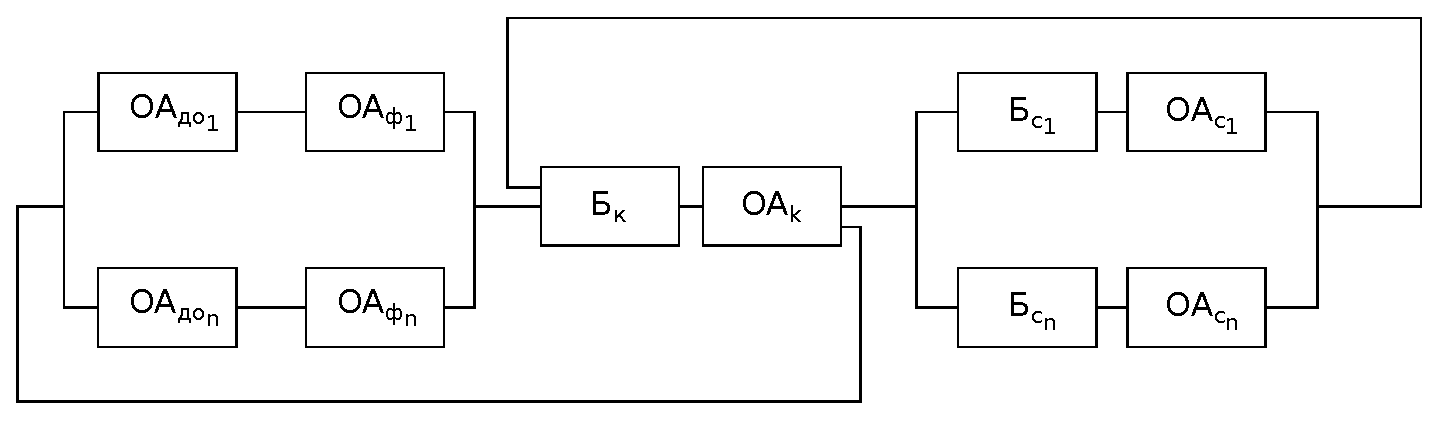
\includegraphics[width=1.0\textwidth]{anal2}
\caption{Формализованная схема рассматриваемой модели (ПЭВМ, канал и два сервера)}
\label{fig:anal-2}
\end{figure}

На схеме~\ref{fig:anal-2} используются следующие обозначения:
\begin{itemize}[label=-]
\item $OA_{\text{до}_i}$ - обслуживающий аппарат, имитирующий дообработку на $i$-ой рабочей станции сети запроса от этой станции к серверу после обработки запроса на сервере;
\item $OA_{\text{ф}_i}$ - обслуживающий аппарат, имитирующий формирование запроса от $i$-ой рабочей станции к серверу;
\item $\text{Б}_\text{к}$ - буфер, имитирующий очередь запросов к каналу;
\item $OA_\text{к}$ - обслуживающий аппарат, имитирующий задержку при передаче данных в канале;
\item $\text{Б}_{\text{с}_i}$ - буфер, имитирующий очередь запросов к $i$-ому серверу;
\item $OA_{\text{с}_i}$ - обслуживающий аппарат, имитирующий работу $i$-ого сервера.
\end{itemize}

\begin{longtable}{p{2cm}|p{15cm}}
\caption{Исходные данные модели}
\label{tab:anal-input} 
\\
Параметр & Описание \\
\hline
$T_o$ & Среднее время дообработки на рабочей станции сети запроса от этой станции к серверу \\
$T_p$ & Среднее время формирования запроса от рабочей станции сети к серверу \\
$t_k$ & Среднее значение времени передачи запроса по каналу \\
$m$   & Число серверов \\
$n$   & Число рабочих станций в сети \\
$t_s$ & Среднее время обработки запроса в сервере
\end{longtable}

\clearpage
\begin{longtable}{p{2cm}|p{15cm}}
\caption{Выходные данные модели}
\label{tab:anal-input} 
\\
Параметр & Описание \\
\hline
$T_\text{реак}$ & Среднее время реакции системы \\
$\rho_{pc}$ & коэффициент загрузки ОА, имитирующего работу рабочей станции сети \\
$\rho_k$ & коэффициент загрузки ОА, имитирующего работу канала передачи данных \\
$\rho_{\text{с}_i}$ & коэффициент загрузки ОА, имитирующего работу $i$-ого сервера \\
\end{longtable}

\subsection{Аналитическое моделирование}
Введем следующие обозначения:
\begin{itemize}[label=-]
\item $\lambda_{\text{ф}_i}$ - среднее значение суммарной интенсивности фонового потока запросов, выходящих из ОА, имитирующих работу рабочих станций, в канал (на $i$-ом шаге алгоритма);
\item $t_k = \frac{t_{k1} + t_{k2}}{2}$ - среднее время обработки запроса в канале передачи данных, где $t_{k1}$ и $t_{k2}$ - соответственно среднее время передачи запроса по каналу в прямом и обратном направлениях;
\item $P_i = \frac{1}{m}$ - вероятность обращения к $i$-ому серверу.
\end{itemize}

При расчете используется приближенный итерационный алгоритм нахождения значения выходных характеристик рассматриваемой системы.

\begin{enumerate}[label=\arabic*)]
\item Определяем начальное значение для $\lambda_{\text{ф}_i}$:
$$
\lambda_{\text{ф}_i} = K_1 \min \left\{ \frac{1}{2t_k}, \frac{1}{P_i t_s} \right\} \frac{n - 1}{n}, \; K_1 \in [0.995 .. 0.99995]
$$
Определяем средние времена пребывания запроса в узлах системы (канале, сервере):
$$
T_k = \frac{2t_k}{1 - 2\lambda_{\text{ф}_i}t_k}
$$

$$
T_s = \frac{t_s}{1 - P_i \lambda_{\text{ф}_i} t_s}
$$

\item Определяем интенсивность фонового потока после очередной итерации:
$$
\lambda_{\text{ф}_{i+1}}' = \frac{n+1}{T_o + T_p + T_k + T_s}
$$

\item Сравниваем $\lambda_{\text{ф}_i}$ и $\lambda_{\text{ф}_{i+1}}'$. Если:
$$
    \frac{| \lambda_{\text{ф}_i} - \lambda_{\text{ф}_{i+1}}' |}{\lambda_{\text{ф}_i}} < \delta
$$
То переходим на пункт 5, иначе на пункт 4;

\item Определяем новое приближенное значение для $\lambda_{\text{ф}_i}$:
$$
\lambda_{\text{ф}_{i+1}} = \lambda_{\text{ф}_i} - \frac{\lambda_{\text{ф}_i} - \lambda_{\text{ф}_{i+1}}'}{K_2}, \; K_2 \in [10 .. 1000]
$$
Переход на пункт 2.

\item Определяем выходные результаты аналитической модели:
$$
T_\text{цикла} = T_o + T_p + T_k + T_s
$$

$$
\lambda = \frac{N}{T_\text{цикла}}
$$

Определяем загрузку основных узлов системы:

Рабочая станция:
$$
    \rho_{pc} = \frac{T_o + T_p}{T_\text{цикла}}
$$

Пользователя:
$$
    \rho_\text{польз} = \frac{T_p}{T_\text{цикла}}
$$

Канала передачи данных:
$$
    \rho_k = 2 \lambda t_k
$$

Сервера:
$$
    \rho_s = \lambda P_i t_s
$$
\end{enumerate}

Результаты аналитического моделирования представлены в таблице~\ref{tab:anal-result}.

\begin{longtable}{p{10cm}|p{1cm}|p{1cm}|p{1cm}|p{1cm}|p{1cm}}
\caption{Результаты аналитического моделирования}
\label{tab:anal-result} \\
\hline
\multicolumn{6}{c}{Проведенные эксперименты} \\ \hline
                                                    & 1      & 2      & 3      & 4      & 5       \\ \cline{2-6}
Количество рабочих станций                          & 8      & 8      & 8      & 8      & 8      \\
Среднее время дообработки запроса на PC             & 80     & 160    & 240    & 160    & 80     \\
Среднее время формирования запроса на PC            & 80     & 160    & 240    & 160    & 80     \\
Количество серверов                                 & 2      & 2      & 2      & 2      & 2      \\
Среднее время обработки запроса на сервере          & 10     & 20     & 20     & 10     & 20     \\
Среднее время передачи запроса по каналу            & 10     & 20     & 20     & 10     & 20     \\  
\hline
\multicolumn{6}{c}{Результаты моделирования} \\ 
\hline
Среднее время реакции системы                       & 225    & 450    & 580    & 364    & 362    \\
Коэффициент загрузки рабочей станции                & 0.71   & 0.71   & 0.83   & 0.88   & 0.44   \\
Коэффициент загрузки канала передачи данных         & 0.71   & 0.71   & 0.55   & 0.44   & 0.88   \\
Коэффициент загрузки сервера                        & 0.18   & 0.18   & 0.14   & 0.11   & 0.22   \\
Коэффициент загрузки пользователя                   & 0.36   & 0.36   & 0.41   & 0.44   & 0.22   \\
\end{longtable}

\subsection{Имитационное моделирование}
\subsection{Сравнительный анализ результатов моделирования}

\clearpage
\section{Выводы}

\clearpage
\section{Литература}


\end{document}